\documentclass[twoside]{ltjsreport}
\usepackage[top=20truemm,bottom=20truemm,left=15truemm,right=15truemm,headheight=20pt]{geometry}
\usepackage{fancyhdr,lastpage,abstract,listings,float,wrapfig,tabularx,multirow}
\usepackage{hyperref,graphics,graphicx,framed}
\usepackage[symbol]{footmisc}
\usepackage{amsmath,amssymb}
\usepackage{tikz}
\usetikzlibrary{calc,arrows.meta,fit}
\newcolumntype{A}{>{\centering\bfseries}X}
\newcolumntype{B}{>{\centering\bfseries\arraybackslash}X}
\newcolumntype{C}{>{\centering\arraybackslash}X}
\newcolumntype{R}{>{\raggedright\arraybackslash}X}
\newcolumntype{L}{>{\raggedleft\arraybackslash}X}
\bibliographystyle{junsrt}
\hypersetup{
    colorlinks=true,
    citecolor=black,
    linkcolor=black,
    urlcolor=red
}
\renewcommand{\chaptermark}[1]{\markboth{第\ \thechapter\ 章\,\, #1}{}}
\fancypagestyle{report}{
    \fancyhf{}
    \fancyhead[RO,LE]{\leftmark}
    \fancyfoot[RO,LE]{\thepage\ /\ \pageref{LastPage}}
    \pagenumbering{arabic}
    }
\fancypagestyle{appendixstyle}{
    \fancyhf{}
    \fancyhead[RO,LE]{付録}
    \fancyfoot[RO,LE]{\thepage\ /\ \pageref{LastPage}}
    \renewcommand{\headrulewidth}{0mm}
}
\lstset{
    language = {Matlab},
    %backgroundcolor={\color[gray]{.90}},
    breaklines = true,
    breakindent = 10pt,
    basicstyle = \ttfamily\small,
    commentstyle = {\ttfamily \color[cmyk]{1,0.4,1,0}},
    classoffset = 0,
    keywordstyle = {\bfseries \color[cmyk]{0,1,0,0}},
    stringstyle = {\ttfamily \color[rgb]{0,0,1}},
    frame = single,
    %他オプション:leftline,topline,bottomline,lines,single,shadowbox
    framesep = 5pt,
    numbers = left,
    stepnumber = 1,
    numberstyle = \small,
    tabsize = 4,
    captionpos = t,
    otherkeywords = {soundsc, xticks, yticks, exportgraphics}
}
\renewcommand{\figurename}{}
\renewcommand{\tablename}{}
\renewcommand{\lstlistingname}{}
\renewcommand{\thefootnote}{\fnsymbol{footnote}}
\renewcommand{\contentsname}{目次}
\renewcommand{\listfigurename}{図目次}
\renewcommand{\listtablename}{表目次}
\renewcommand{\lstlistlistingname}{ソースコード}
\renewcommand{\thefigure}{Fig.\thechapter-\arabic{figure}}
\renewcommand{\thetable}{Tbl.\thechapter-\arabic{table}}
\renewcommand{\theequation}{\thechapter.\arabic{equation}}
\renewcommand{\labelenumi}{\textbf{\theenumi}.\ }
\renewcommand{\eqref}[1]{式(\ref{#1})}
\newcommand{\matlab}{{\large M}ATLAB\raisebox{2mm}{\tiny\textregistered}}
\newcommand{\mat}[2]{\(#1\)行\(#2\)列}
\newcommand{\srcref}[2]{\ref{#1}節ソースコードは\(\underset{\text{\scriptsize\({}_{\Rightarrow\textrm{p.\pageref{#2}}}\)}}{\textrm{\ref{#2}}}\).}
\makeatletter
\@addtoreset{figure}{chapter}
\@addtoreset{table}{chapter}
\@addtoreset{lstlisting}{chapter}
\@addtoreset{footnote}{page}
\renewcommand{\chapter}{%
    \if@openright\cleardoublepage\else\clearpage\fi
    \global\@topnum\z@
    \secdef\@chapter\@schapter}
\makeatother
\AtBeginDocument{
    \renewcommand{\thelstlisting}{src.\thechapter-\arabic{lstlisting}}
}
\title{音の工学的特徴とそれに対する聴覚の特性についての考察}
\author{溝口 洸熙\thanks{高知工科大学 情報学群 学籍番号:1250373 Group10}}
\date{May 7th, 2023}
\begin{document}
% paragraph command
\newcommand{\purpose}{\subsection{実験の目的}}
\newcommand{\method}{\subsection{実験の方法と考え方}}
\newcommand{\result}{\subsection{実験の結果}}
\newcommand{\consideration}{\subsection{考察}}
\newcommand{\conclusion}{\subsection{結論}}
% 課題1
\newcommand{\kadaiaa}{カラーチャネル操作}
\newcommand{\kadaiab}{画像の量しかビット数変換}
\newcommand{\kadaiac}{階調反転}
\newcommand{\kadaiad}{閾値処理}
\newcommand{\kadaiae}{ヒストグラム}
% 課題2
\newcommand{\kadaiba}{テスト画像作成}
\newcommand{\kadaibb}{平滑化フィルタ・メディアンフィルタ}
\newcommand{\kadaibc}{微分フィルタ}
\newcommand{\kadaibd}{ラプラシアンフィルタ}
\newcommand{\kadaibe}{色空間変換}
\maketitle
\renewcommand{\abstractname}{概要}
\begin{abstract}
    本実験では,画像情報処理,視覚情報処理を扱う.画像情報処理では,カラーチャネル操作や閾値処理,量子化数変換などの基礎的な画像処理を行い,それらの技術を用いて画像フィルタや背景差分画像の作成や肌色領域の抽出,2次元フーリエ変換を行う.2次元フーリエ変換のパワースペクトルと原画像の関係や,2次元フーリエ変換後の出力と,画像座標との関係が明らかになった.また,背景差分画像と色空間変換後の肌色領域抽出で,対象物の抽出における特徴も明らかとなった.
    視覚情報処理では,方位残効を扱う.\matlab 上で方位残効刺激を作成する.この実験より,縞模様方位の大きさと,方位残効の度合いの関係を,ヒトの視覚情報処理を考慮した上で明らかになった.
\end{abstract}
\pagenumbering{roman}\thispagestyle{plain}
\tableofcontents
\listoffigures
\listoftables
\lstlistoflistings
\newpage
\pagestyle{report}
\setcounter{page}{1}
% \chapter{音の工学的特徴}
\section{\kadaiaa}\label{sec:\kadaiaa}
\purpose
我々は音の「高い」「低い」をどのようにして認識しているのだろうか.音が高いまたは低いと感じるためには何かと比較するはずだがその比較の指標は何だろうか.
この実験ではまず,正弦波の生成をプログラミングを用いて作成する.そして周波数の変化に対して正弦波グラフおよび音の違いを実験を通して確認し,考察する.
\method
\paragraph{実験に用いる装置}このレポート内全ての実験に用いる言語はMathWorks\raisebox{2mm}{\tiny\textregistered}社の\matlab を用い,\ref{tbl:実験環境}の環境を用いて実験する..
\begin{table}[H]
    \caption{実験環境}
    \label{tbl:実験環境}
    \begin{tabularx}{\textwidth}{AR}
        \hline
        実験機                   & Mac Studio 2022 (Apple社)    \\
        プロセッサ               & Apple Silicon M1 Max           \\
        メモリ                   & 32GB                           \\
        \multirow{2}{*}{\matlab} & R2023a Update1 9.14.02239454   \\
                                 & 64-bit (maci64) March 30, 2023 \\
        \hline
    \end{tabularx}
\end{table}
また,このレポートない全ての実験では\matlab でプロットしたグラフを出力するために,関数\ref{src:グラフ出力}を用いている.
\begin{lstlisting}[numbers={none},caption={グラフ出力},label={src:グラフ出力}]
exportgraphics(figurename,'path/figure_name.pdf','ContentType','vecto')
\end{lstlisting}
\paragraph{正弦波について}時刻\(t\)に対して周波数\(f\)の正弦波は,\eqref{equ:正弦波}で得られる.
\begin{align}
    y & =\sin(2\pi ft)\label{equ:正弦波}
\end{align}
時間軸データ\(t\)を\mat{1}{N}のベクトルに代入する.
時間軸データの作成について,サンプリング周波数\texttt{Fs}に対して\(m\)秒間の正弦波を生成するためには,\ref{src:時間軸作成と正弦波の作成}のように\texttt{0}から\texttt{Fs}まのベクトルに対して,各要素をサンプリング周波数で割ると時間軸テーブルを作成することができる.\par
\begin{wrapfigure}{r}[0mm]{.4\textwidth}
    \begin{lstlisting}[caption={時間軸作成と正弦波の作成},numbers={none},label={src:時間軸作成と正弦波の作成}]
t = (0 : m*(Fs-1)) /Fs;
y = sin(2*pi*f*t);
\end{lstlisting}
\end{wrapfigure}
\(t\)の各要素\(t_n\)に対して三角関数\(\sin(2\pi ft_n)\)を演算し,ベクトル\(y\)の要素\(y_n\)に代入する.従って\(y\)も\mat{1}{N}のベクトルになる.
生成した正弦波を\texttt{plot}関数を用いて\(y\)を\(t\)の関数として描画する.このように,ただ一つの正弦波からなるような音を\textbf{純音}という.\cite[p.1]{音響工学理論基礎}
また,サンプリング周波数を\texttt{Fs}とし,データ列\texttt{y}を再生するためには\texttt{sound}関数を用いる.\par
\paragraph{実験内容}この実験では,周波数を\(f_1=440\textrm{Hz}\),\(f_2=660\textrm{Hz}\)の2種類を用いてそれぞれ正弦波\(y_1\),\(y_2\)を生成する.生成した\(y_n(n=\{1,2\})\)に対して,\(t\)を横軸に取りグラフを作成し,サンプリング周波数を\(\textrm{\texttt{Fs}}=16000\textrm{Hz}\)として再生する.\srcref{sec:\kadaiaa}{src:01_01}
\result
各正弦波のグラフを\ref{fig:\kadaiaa}に示す.音を聴き比べた結果,\(f_2\)の周波数を用いた正弦波は\(f_1\)を用いた正弦波に比べて音が高かった.具体的には\(f_1\)がAの音\footnote{イタリア語音階で「ラ」}であるのに対して,\(f_2\)の音は完全5度大きいEの音\footnote{イタリア語音階で「ミ」}であった.
\begin{wrapfigure}{r}[0mm]{.3\textwidth}
    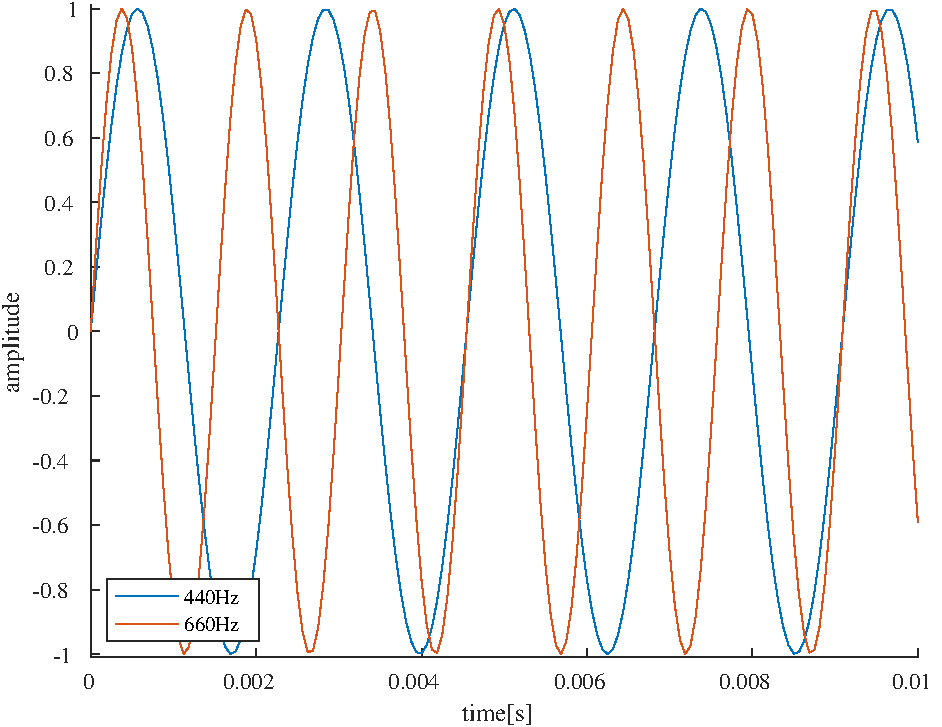
\includegraphics[keepaspectratio,width=.3\textwidth]{../../Figures/01_01.pdf}
    \caption{周波数が異なる正弦波のグラフ}
    \label{fig:\kadaiaa}
\end{wrapfigure}
さらに,聴音確認・目視確認では音の大きさ,音色,振幅や波形の変化は確認でなかった.\par
\consideration 周波数\ \((f)\)\ とは1秒間の振動回数であり,これが音の高さを決める.実験結果より周波数が大きい,つまり1秒間により多く振動すれば音が高くなることが分かった.
また,1回振動あたりの時間を周期\ \((T)\)\ と言うが,周期と周波数は反比例の関係であり,\eqref{equ:周期と周波数}が成り立つ.
\begin{align}
    f & =\frac{1}{T} & \big(\textrm{無論}\quad T\neq 0,\quad f\neq 0\big)\label{equ:周期と周波数}
\end{align}
\ref{fig:周波数の異なる純音の生成}より,周波数が大きい正弦波は周期が短く,逆もまた確認できる.
周波数のみを変更したので,振幅や正弦波の波形変化はない.\par
また,周波数が\(f_1\)正弦波の音と\(f_2\)正弦波の音はそれぞれ純音だがこれらの間にも関係がある.数学的には\(f_1:f_2=2:3\)の簡単な整数比になっている.
\begin{leftbar}
    ヒトの耳は2つの音を同時に聞いた場合,その2つの音の周波数が簡単になっているほど協和して聴こえる.(略)\par
    このように周波数比が整数比になっている音程を純音程とよぶ.\hfill{\cite[p.46-p.47]{音響工学理論基礎}}
\end{leftbar}
つまり,周波数\(f_1\)正弦波と周波数\(f_2\)正弦波の加算合成波はは協和してきこえる.
\section{\kadaiab}\label{sec:\kadaiab}
\purpose
音の大小は何によって決まるのだろうか.音の大小に関わる波の振幅や,波を構成する上で重要な初期位相を変化させ,変化の前後での音の違いを聞き取り,人間の耳に初期位相の変化や振幅の変化がどのように感じるか実験を通して考察する.
\method
時刻\(t\)に対して周波数\(f\)の正弦波は\eqref{equ:正弦波}で得られるが,その初期位相(\textit{initial phase})を\(\phi\)とすると,その正弦波は\eqref{equ:正弦波_初期位相}となる.
\begin{align}
    y & =\sin(2\pi ft+\phi)\label{equ:正弦波_初期位相}
\end{align}また,同様な正弦波:\eqref{equ:正弦波}の振幅を\(A\)倍して得られる正弦波は\eqref{equ:正弦波_振幅}となる.
\begin{align}
    y & =A\sin(2\pi ft)\label{equ:正弦波_振幅}
\end{align}
\begin{wrapfigure}{r}[0mm]{.4\textwidth}
    \begin{lstlisting}[caption={左右から別の音を出力},label={src:左右から別の音を出力},numbers={none}]
Fs = 16000; % サンプリング周波数
y1 = 音声データ1; % N行1列(左)
y2 = 音声データ2; % N行1列(右)
y = [y1 y2]; % N行2列 列結合を行う
sound(y, Fs); 
    \end{lstlisting}
\end{wrapfigure}
\paragraph{実験内容}この実験では,初期位相の変化と振幅の変化,それぞれ実験し変化前と変化後の音や波形の違いを発見する.周波数は\(f=440\textrm{Hz}\)とし,サンプリング周波数を\(\texttt{Fs}=16000\textrm{Hz}\)とする.
左から純音,右から波長や初期位相を変化させた音を再生するようにして(\ref{src:左右から別の音を出力}),音の変化を確認する.\srcref{sec:\kadaiab}{src:01_02}
\begin{table}[h]
    \caption{\kadaiab\ 実験内容}
    \label{tbl:\kadaiab_実験内容}
    \begin{tabularx}{\textwidth}{RCCR}
        \multicolumn{1}{c}{\textbf{実験対象}} & \multicolumn{1}{c}{\textbf{振幅(基準倍)}} & \multicolumn{1}{c}{\textbf{初期位相}} & \multicolumn{1}{c}{\textbf{生成される正弦波}} \\
        \hline
        純音                                  & 基準                                        & 基準                                  & \(y_0=\sin(2\pi ft)\)                         \\
        \hline
        \multirow{2}{*}{振幅}                 & \(0.5\)                                     & \(0\)                                 & \(y_1=0.5\times\sin(2\pi ft)\)                \\
                                              & \(0.25\)                                    & \(0\)                                 & \(y_2=0.25\times\sin(2\pi ft)\)               \\
        \hline
        \multirow{2}{*}{初期位相}             & \(1\)                                       & \(+\frac{\pi}{2}\)                    & \(y_3=\sin(2\pi ft+\frac{\pi}{2})\)           \\
                                              & \(1\)                                       & \(+\pi\)                              & \(y_4=\sin(2\pi ft+\pi)\)                     \\
        \hline
    \end{tabularx}
\end{table}
\result
聴音確認の結果を\ref{tbl:\kadaiab_実験結果},\ref{fig:振幅・位相の確認_結果_振幅}及び\ref{fig:振幅・位相の確認_結果_初期位相}に示す.振幅の変化について,振幅の変化に比例した音量変化を確認できたが,初期位相の変化による音の変化は確認できなかった.
\begin{table}[H]
    \caption{\kadaiab\ 実験結果}
    \label{tbl:\kadaiab_実験結果}
    \begin{tabularx}{\textwidth}{ccclR}
        \multicolumn{1}{c}{\textbf{実験対象}} & \multicolumn{1}{c}{\textbf{振幅(基準倍)}} & \multicolumn{1}{c}{\textbf{初期位相}} & \multicolumn{1}{c}{\textbf{生成される正弦波}} & \multicolumn{1}{c}{\textbf{純音との比較}} \\
        \hline
        純音                                  & 基準                                        & 基準                                  & \(y_0=\sin(2\pi ft)\)                         & \multicolumn{1}{c}{---}                   \\
        \hline
        \multirow{2}{*}{振幅}                 & \(0.5\)                                     & \(0\)                                 & \(y_1=0.5\times\sin(2\pi ft)\)                & 音量がおおよそ\(1/2\)に聞こえた.         \\
                                              & \(0.25\)                                    & \(0\)                                 & \(y_2=0.25\times\sin(2\pi ft)\)               & 音量がおおよそ\(1/4\)に聞こえた.         \\
        \hline
        \multirow{2}{*}{初期位相}             & \(1\)                                       & \(+\frac{\pi}{2}\)                    & \(y_3=\sin(2\pi ft+\frac{\pi}{2})\)           & 違いは分からなかった.                    \\
                                              & \(1\)                                       & \(+\pi\)                              & \(y_4=\sin(2\pi ft+\pi)\)                     & 違いは分からなかった.                    \\
        \hline
    \end{tabularx}
\end{table}
\begin{figure}[H]
    \centering
    \begin{minipage}[b]{.48\textwidth}
        \centering
        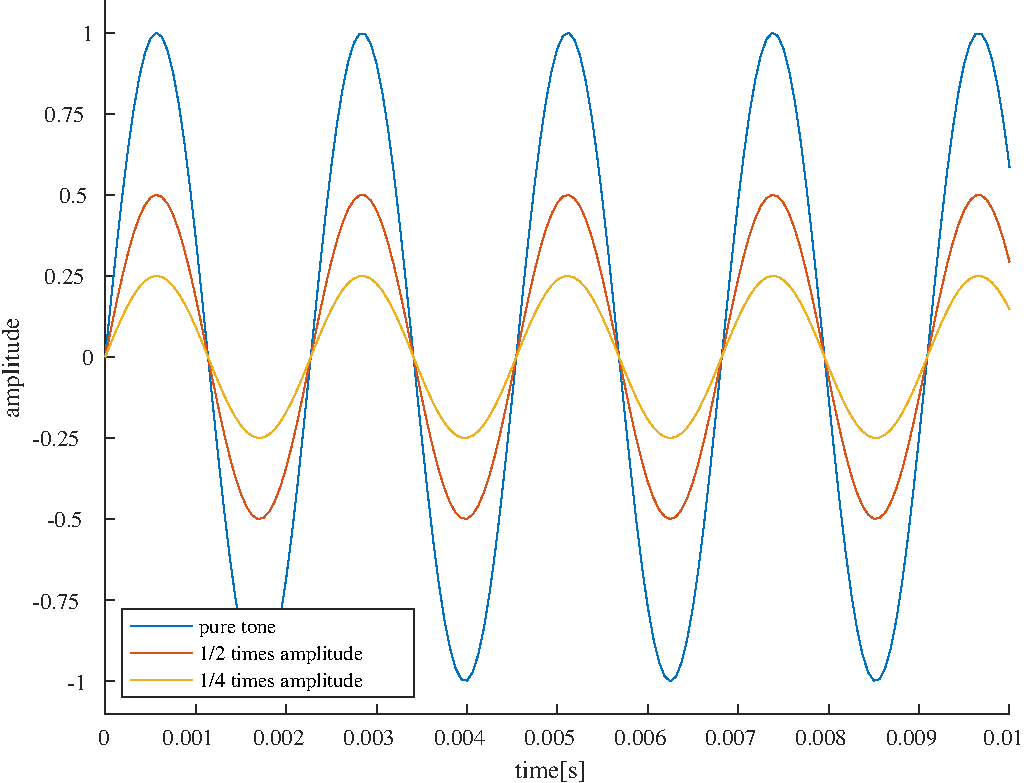
\includegraphics[keepaspectratio,width=\textwidth]{../../Figures/01_02_1.pdf}
        \caption{\kadaiab\ 実験結果(振幅の変化)}
        \label{fig:\kadaiab_結果_振幅}
    \end{minipage}
    \begin{minipage}[b]{.48\textwidth}
        \centering
        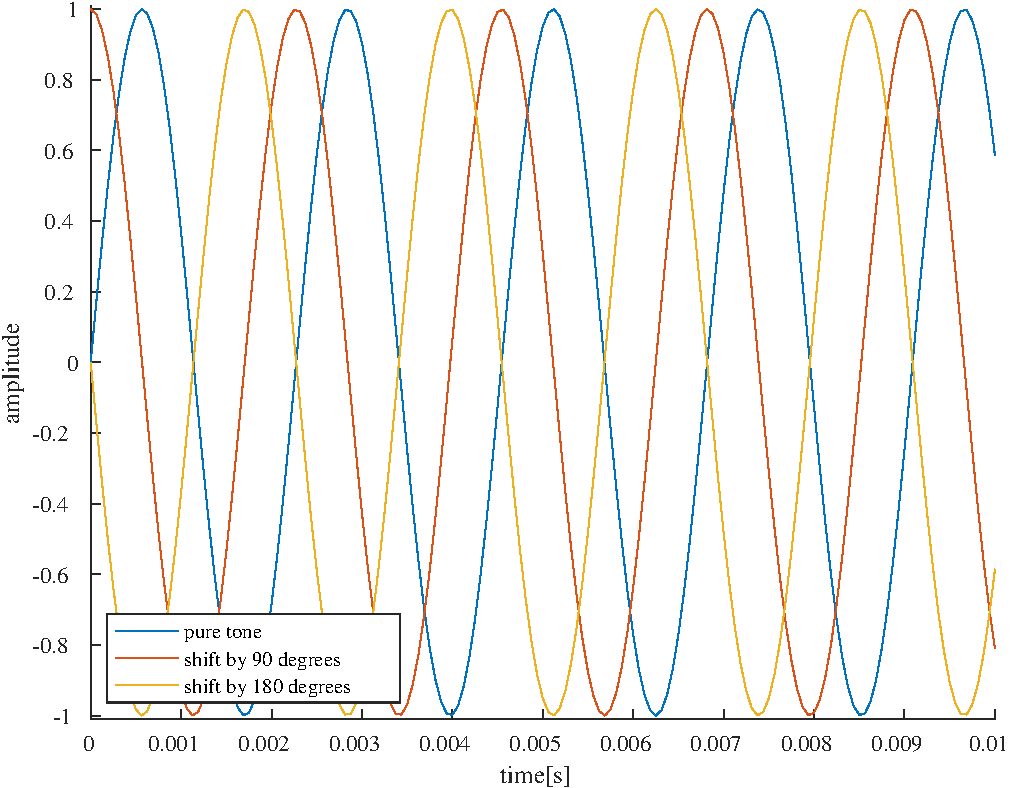
\includegraphics[keepaspectratio,width=\textwidth]{../../Figures/01_02_2.pdf}
        \caption{\kadaiab\ 実験結果(初期位相の変化)}
        \label{fig:\kadaiab_結果_初期位相}
    \end{minipage}
\end{figure}
\consideration
\paragraph{振幅の変化について} 振幅の変化は,音量と比例することを確認できた.\ref{fig:振幅・位相の確認_結果_振幅}より,各正弦波において周期や初期位相が等しいので,縦軸が\(0\)になる時刻や最大値を迎えるは等しいく,振幅のみが異なる.
\paragraph{初期位相の変化について} 位相の変化による音の変化は確認できなかった.\ref{fig:振幅・位相の確認_結果_初期位相}より,振幅や周期は等しいが,初期位相が異なるため最小値や最大値を迎える時刻が初期位相分異なる.
\section{\kadaiac}\label{sec:\kadaiac}
\purpose
ティンパニやギターのチューニングを行うとき,音叉やチューナーから音を出して,異なる互いに周波数であれば気づきチューニングする.それぞれ異なる周波数が異なる周波数が周波数の違いによるうなりの発生やその原因を数学的観点から考察する.
\method
うなりとは,異なる周波数が干渉するとき起こる現象である.異なる周波数同士の正弦波が干渉することで,強め合いの場所と弱め合いの場所が周期的に現れることで発生する.
例えば周波数\(f_1\)の正弦波に対して周波数\(f_2(\neq f_1)\)の正弦波を干渉させると,\eqref{equ:うなり}より\(1\)秒間に\(N\)回のうなりを聞くことができる.
\begin{align}
    N & = \big|f_1-f_2\big|\label{equ:うなり}
\end{align}
\(f_1\)と\(f_2\)の差が大きければ,当然うなり(\(N\))の回数は多くなり,\(f_1\)と\(f_2\)の差が小さければうなりの回数は少なくなる.\par
本実験では,サンプリング周波数を\(\texttt{Fs}=16000\textrm{Hz}\),提示時間\(4\)秒,周波数が\(f_1=440\textrm{Hz}\)の純音\(y_1\),\(f_2=441\textrm{Hz}\)の純音\(y_2\)を加算合成\(\big(y_1+y_2\big)\)した波形を生成し再生する.\srcref{sec:\kadaiac}{src:01_03}
\begin{wrapfigure}{r}[0mm]{.3\textwidth}
    \centering
    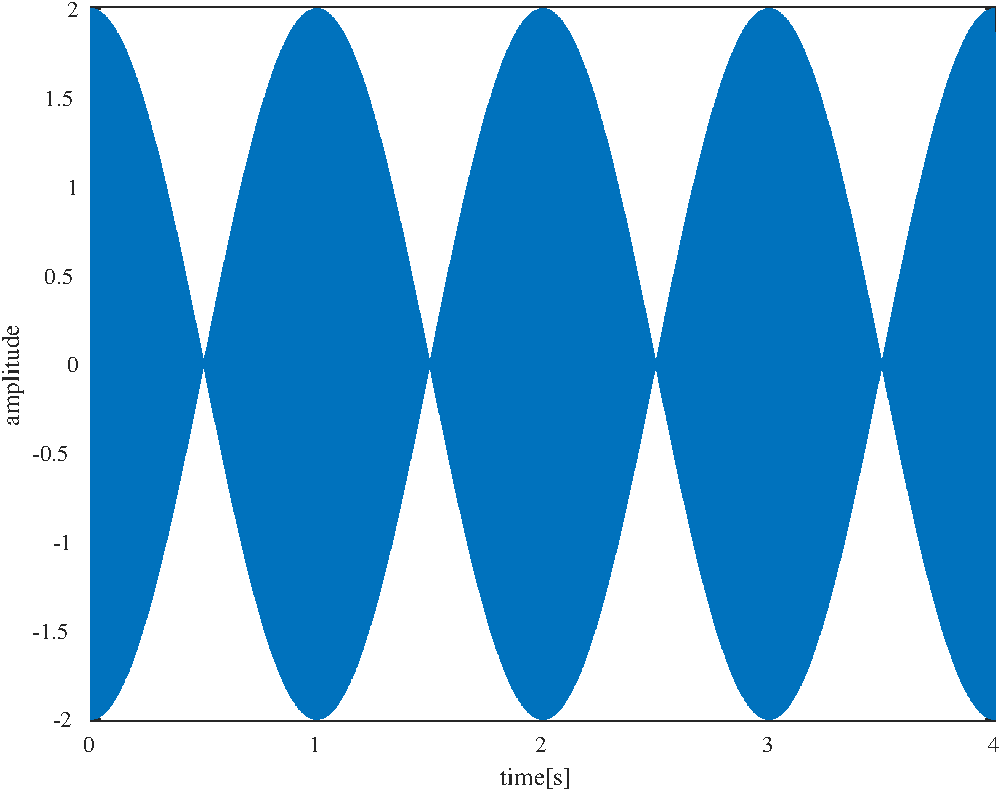
\includegraphics[keepaspectratio,width=.3\textwidth]{../../Figures/01_03.pdf}
    \caption{\kadaiac\ 実験結果}
    \label{fig:\kadaiac_実験結果}
\end{wrapfigure}
\result
うなりは4回聞こえた.また,時間軸に対して加算合成したデータを描画すると\ref{fig:\kadaiac_実験結果}となった.
\consideration \eqref{equ:うなり}に従って,
\begin{equation}
    \begin{aligned}
        \big|f_1-f_2\big| & = \big|440-441\big| \\
                          & =1
    \end{aligned}
\end{equation}
より\(1\)秒あたり\(1\)回のうなりが聞こえるはずなので,この実験結果は論理的に正しい.
加算合成波\ref{fig:\kadaiac_実験結果}の振幅に着目しても,周波数\(f_1\),\(f_2\)それぞれの正弦波の振幅が1であることを考えると,その加算合成波の振幅が2であることも理解できる.
さらに,この加算合成波は\(t=0\)のとき最大値を迎えており,これは初期位相が同一の正弦波の加算合成であることを表している.
\section{\kadaiad}\label{sec:\kadaiad}
\purpose
矩形波は周期関数だが,見た目は正弦波ではない.これをプログラム上でどのように再現するのか.フーリエ級数展開を用いた矩形波の描画やフーリエ級数展開のプログラム上で再現し,理想的な矩形波との比較を行う.
\method
\paragraph{フーリエ級数展開}周期\(T\)の任意の周期信号\(f(t)\)に対して,それはより短い周期\(T/n(n=1,2,\dots)\)を持つ正弦波の重ね合わせで表すことができる.具体的には\eqref{equ:フーリエ級数展開}の\(N=\infty\)で表すことができ,これをフーリエ級数展開という.\cite[p.18-p.19]{信号処理}特に\eqref{equ:フーリエ級数展開}の\(N=1\)の時を基本周波数と呼ぶ.
また,\(k>1\)のときの周波数を持つ正弦波を高調波と呼ぶ.

\begin{wrapfigure}{r}[0cm]{.3\textwidth}
    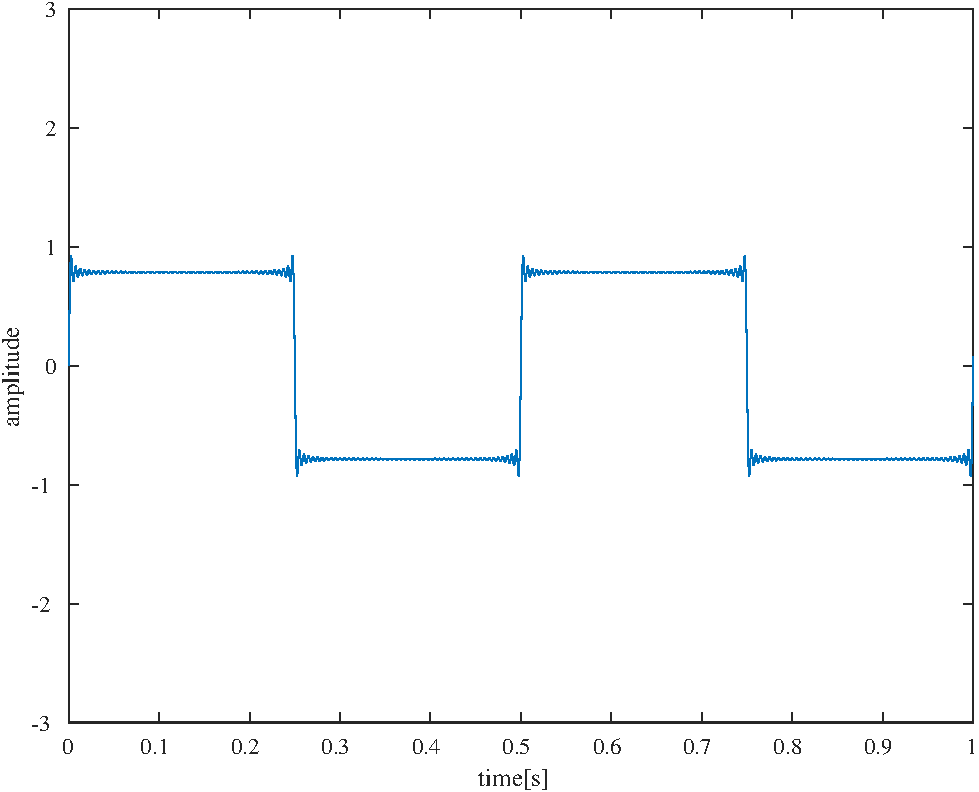
\includegraphics[keepaspectratio,width=.3\textwidth]{../../Figures/01_04_1.pdf}
    \caption{矩形波(\(1\leq k\leq 50\))}
    \label{fig:矩形波}
\end{wrapfigure}
\begin{align}
    f(t) & =\frac{1}{2}a_0 + \sum_{k=1}^{N}\big(a_k\cos(k\omega_0t)+b_k\sin(k\omega_0t)\big) & \omega_0 & =\frac{2\pi}{T}\label{equ:フーリエ級数展開}
\end{align}
\paragraph{矩形波}
矩形波は周期関数である.その周期を\(T\)とすると,関数\(f\)は時刻\(t\)に対して,フーリエ級数展開するとになる.\eqref{equ:矩形波}\((N=\infty)\)は周期\(T=1/2\)で定義した矩形波で,\eqref{equ:矩形波}を\(N=50\)で出力した.
\begin{align}
    f(t) & =\sum_{k=1}^{N}\frac{1}{2k-1}\sin\big(2\pi(2k-1)ft\big)\label{equ:矩形波}
\end{align}
\paragraph{実験内容}周期\(T=1/2\)として,\eqref{equ:矩形波}の\(N\)の値を\(N=1, 5, 25\)と増やした時に次第に波形が矩形波に収束していくことを確認する.
計算機で和\(\big(\sum\big)\)の演算をに示す通りに行う.\srcref{sec:\kadaiad}{src:01_04}
\begin{lstlisting}[caption={和の演算},label={src:和の演算},numbers={none}]
y = 0;
for k=1:50
    y = y + 1/(2*k-1) * sin(2*pi*(2*k-1)*f*t); % 矩形波の例
end
\end{lstlisting}
\result
\begin{wrapfigure}{r}[0mm]{.3\textwidth}
    \centering
    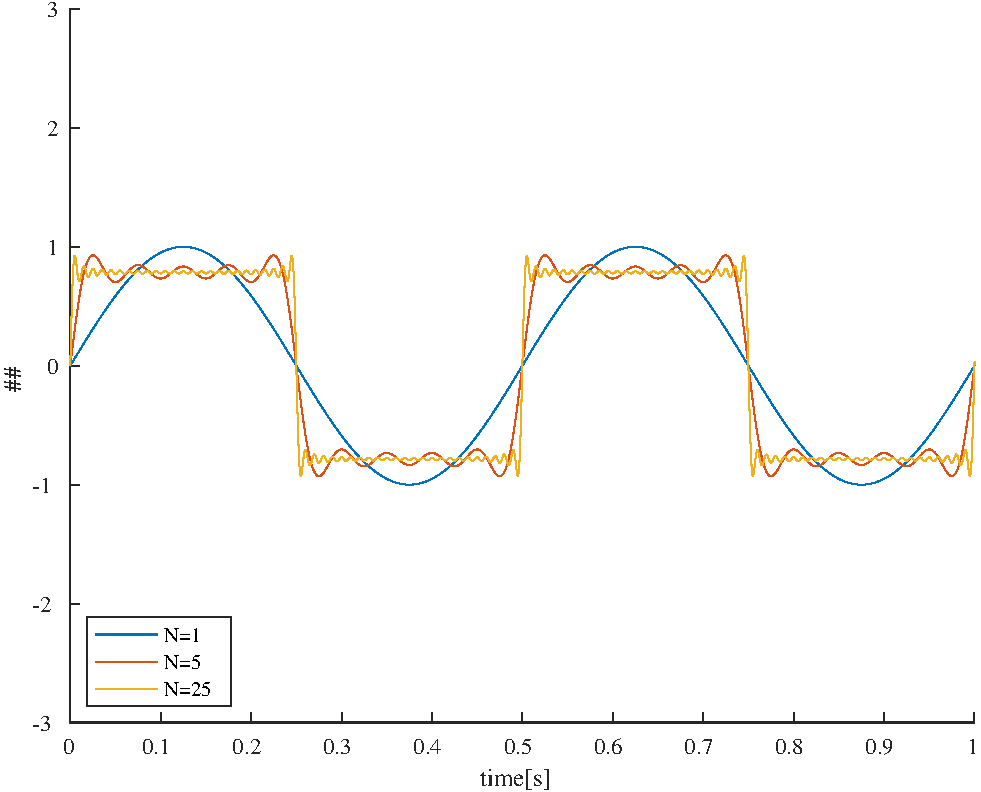
\includegraphics[keepaspectratio,width=.3\textwidth]{../../Figures/01_04_2.pdf}
    \caption{\kadaiad\ 実験結果}
    \label{fig:\kadaiae_実験結果}
    \vspace{-1cm}
\end{wrapfigure}
\ref{fig:\kadaiae_実験結果}の通り,\(N\)を大きくすると,矩形波に収束することがわかった.また,基本周波数と矩形波の周期も目測では一致している.
\consideration
計算機を用いて\(N\)の値を無限大で出力することは不可能である.\ref{fig:矩形波}のように\(N=50\)として出力すると,理想的な矩形波に近づくが完全ではない.\par
ここで\(N\)の値を大きくすると,\(T/2, T\)あたりで尖ったもの(ひげ)が確認される.フーリエ級数では不連続で誤差が大きい.このことをギブス現象という.\cite[p.34]{信号処理}
\section{\kadaiae}\label{sec:\kadaiae}
\purpose
白色雑音(\textit{white noise})は以下のように定義されている.
\begin{leftbar}
    すべての周波数成分を均等に含む,パワースペクトルが一定である不規則性の非常に強い波のことである.
    \hfill\cite{witenoise}
\end{leftbar}
ガウス雑音(\textit{gaussian noise})は以下のように定義されている.
\begin{leftbar}
    Gaussian noise represents statistical noise having the probability density function equal to that of the normal distribution.
    \hfill\cite{barbu2013variational}
\end{leftbar}
つまり,「正規分布の確率関数と等しい確率密度関数を持つ統計的ノイズ」を表す.今回の実験ではガウス雑音を計算機上で構成し,その信号振幅のヒストグラムを作成する.そのヒストグラムがガウス分布\footnote{以後,課題内容や他の用語との兼ね合いにより「正規分布」を「ガウス分布」と表す.}に従っているかを確認する.

\begin{wrapfigure}{r}[0mm]{.3\textwidth}
    \vspace{-.5cm}
    \begin{lstlisting}[caption={乱数生成・ヒストグラム},label={src:乱数生成・ヒストグラム},xleftmargin=3mm]
rng(0, 'twister');
X = randn(n,m);
num = 100;
[h, c] = hist(X, num);
plot(c,h);
    \end{lstlisting}
    \begin{lstlisting}[caption={平均と標準偏差の変更},label={src:平均と標準偏差の変更},numbers={none},xleftmargin=3mm]
X = randn(n,m); % 乱数生成
X = a.*X + b; % 演算
    \end{lstlisting}
    \vspace{-1cm}
\end{wrapfigure}
\method
\paragraph{\matlab 関数の説明}標準正規分布から乱数の行列を取り出すには,\texttt{randn}関数を用いる.乱数生成機の初期化を行い,\mat{n}{m}の乱数をを取り出すには,\ref{src:乱数生成・ヒストグラム}[1-2行目]を記述する.
また,データ列\texttt{X}に対して,ヒストグラムを\texttt{num}段階で分割し表示するためには,\ref{src:乱数生成・ヒストグラム}[3-5行目]を記述する.
\paragraph{ガウス分布と標準正規分布}ガウス分布とは,平均値・中央値・最頻値が一致するという特徴を持つ確率分布.その確率変数を\(x\)としたときの確率密度関数\(f\)は\eqref{equ:確率密度関数}のように与えらえる.
標準正規分布は,平均\(\mu=0\),標準偏差\(\sigma^2=1\)のガウス分布である.その標準正規分布の確率密度関数\(f_N\)は\eqref{equ:標準正規分布}となる.
\begin{align}
    f(x)   & = \frac{1}{\sqrt{2\pi\sigma^2}}\exp\left(-\frac{(x-\mu^2)}{2\sigma^2}\right) & \big(\mu:\textrm{平均}\quad\sigma^2:\textrm{分散}\quad-\infty<x<\infty\big)\label{equ:確率密度関数} \\
    f_N(x) & =\frac{1}{\sqrt{2\pi}}\exp\left(-\frac{x^2}{2}\right)                        & \big(-\infty<x<\infty\big)\label{equ:標準正規分布}
\end{align}
\begin{leftbar}
    確率変数\(x\)に対して,その平均が\(\mu_x\),分散が\({\sigma_x}^2\)のとき,\(y=ax+b\quad(a\textrm{と}b\textrm{は定数})\)で定義される確率変数\(y\)の平均は\(\mu_y=a\mu_x+b\),分散は\({\sigma_y}^2=a^2{\sigma_x}^2\)となる.\hfill\cite{matlab}
\end{leftbar}
従って,標準正規分布に従って出力されたデータ列の平均を\texttt{a},標準偏差を\texttt{b}に変更したい場合には,\mat{n}{m}データ列\texttt{X}に対して\texttt{X}の各要素と\texttt{a}の積をとり,データ列\texttt{X}と\texttt{b}の和をとる.(\ref{src:平均と標準偏差の変更})\srcref{sec:\kadaiae}{src:01_05}
\result
ガウス雑音の波形を\ref{fig:ガウス雑音の波形},ヒストグラムを\ref{fig:ヒストグラム}に示す.聴音した結果,「ザー」という所謂雑音が聞こえた.
\begin{figure}[h]
    \centering
    \begin{minipage}[b]{.48\textwidth}
        \centering
        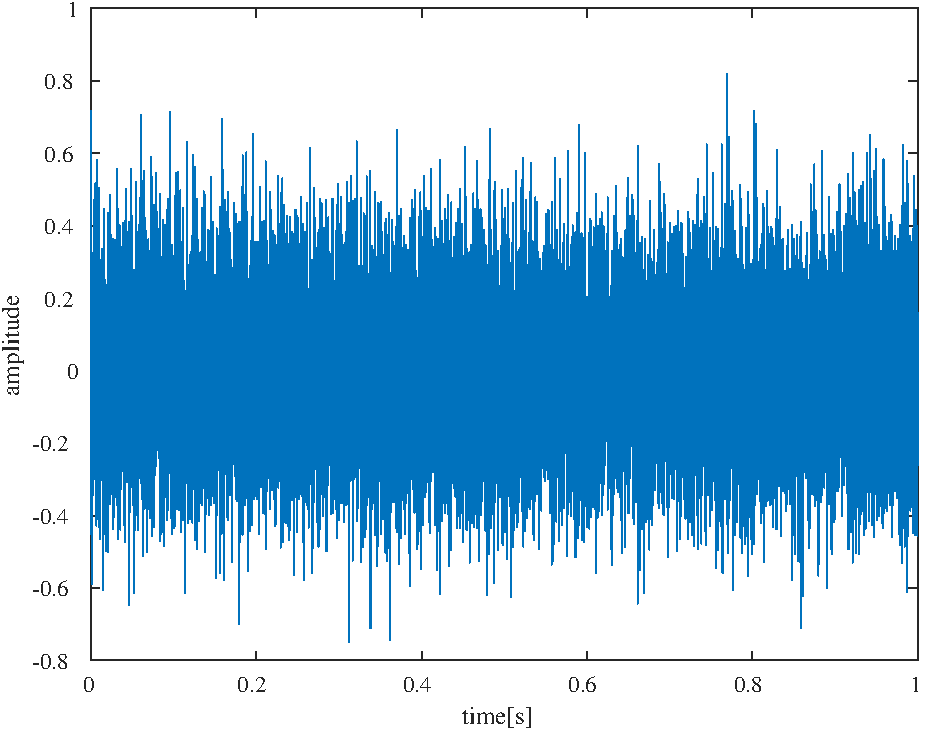
\includegraphics[keepaspectratio,height=.2\textheight]{../../Figures/01_05_0.pdf}
        \caption{ガウス雑音の波形}
        \label{fig:ガウス雑音の波形}
    \end{minipage}
    \begin{minipage}[b]{.48\textwidth}
        \centering
        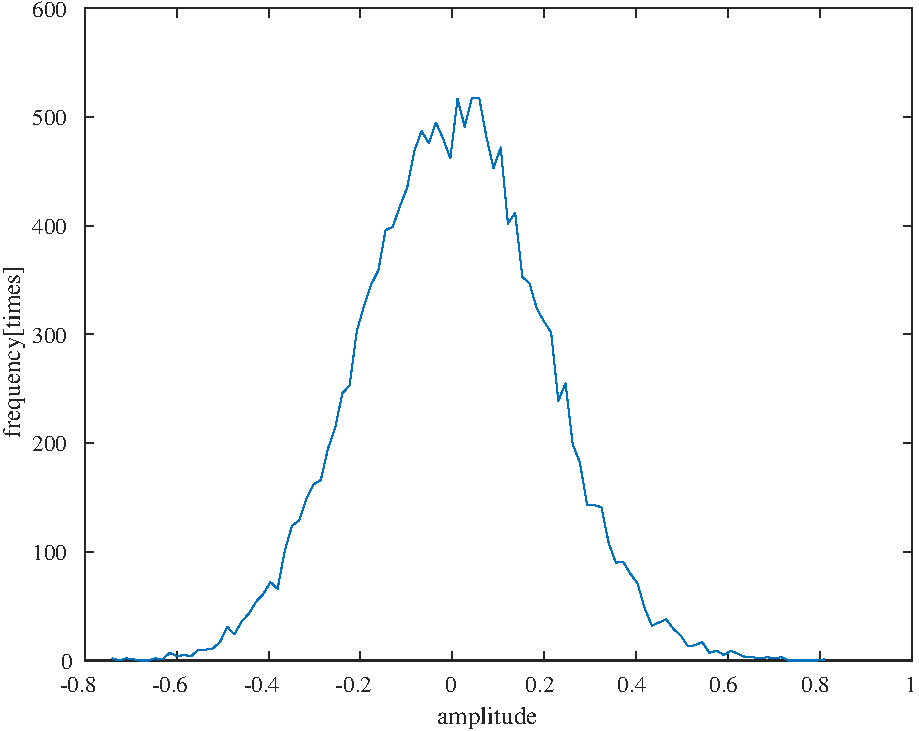
\includegraphics[keepaspectratio,height=.2\textheight]{../../Figures/01_05_1.pdf}
        \caption{ヒストグラム}
        \label{fig:ヒストグラム}
    \end{minipage}
\end{figure}
\consideration
聴音確認による,ガウス雑音の特徴は捉えることができなかった.ヒストグラム\ref{fig:ヒストグラム}を確認すると,平均\(\mu=0\)のガウス分布におおよそ従っていることがわかる.

\chapter{音の工学的特徴}
\section{\kadaiaa}\label{sec:\kadaiaa}
\purpose
我々は音の「高い」「低い」をどのようにして認識しているのだろうか.音が高いまたは低いと感じるためには何かと比較するはずだがその比較の指標は何だろうか.
この実験ではまず,正弦波の生成をプログラミングを用いて作成する.そして周波数の変化に対して正弦波グラフおよび音の違いを実験を通して確認し,考察する.
\method
\paragraph{実験に用いる装置}このレポート内全ての実験に用いる言語はMathWorks\raisebox{2mm}{\tiny\textregistered}社の\matlab を用い,\ref{tbl:実験環境}の環境を用いて実験する..
\begin{table}[H]
    \caption{実験環境}
    \label{tbl:実験環境}
    \begin{tabularx}{\textwidth}{AR}
        \hline
        実験機                   & Mac Studio 2022 (Apple社)    \\
        プロセッサ               & Apple Silicon M1 Max           \\
        メモリ                   & 32GB                           \\
        \multirow{2}{*}{\matlab} & R2023a Update1 9.14.02239454   \\
                                 & 64-bit (maci64) March 30, 2023 \\
        \hline
    \end{tabularx}
\end{table}
また,このレポートない全ての実験では\matlab でプロットしたグラフを出力するために,関数\ref{src:グラフ出力}を用いている.
\begin{lstlisting}[numbers={none},caption={グラフ出力},label={src:グラフ出力}]
exportgraphics(figurename,'path/figure_name.pdf','ContentType','vecto')
\end{lstlisting}
\paragraph{正弦波について}時刻\(t\)に対して周波数\(f\)の正弦波は,\eqref{equ:正弦波}で得られる.
\begin{align}
    y & =\sin(2\pi ft)\label{equ:正弦波}
\end{align}
時間軸データ\(t\)を\mat{1}{N}のベクトルに代入する.
時間軸データの作成について,サンプリング周波数\texttt{Fs}に対して\(m\)秒間の正弦波を生成するためには,\ref{src:時間軸作成と正弦波の作成}のように\texttt{0}から\texttt{Fs}まのベクトルに対して,各要素をサンプリング周波数で割ると時間軸テーブルを作成することができる.\par
\begin{wrapfigure}{r}[0mm]{.4\textwidth}
    \begin{lstlisting}[caption={時間軸作成と正弦波の作成},numbers={none},label={src:時間軸作成と正弦波の作成}]
t = (0 : m*(Fs-1)) /Fs;
y = sin(2*pi*f*t);
\end{lstlisting}
\end{wrapfigure}
\(t\)の各要素\(t_n\)に対して三角関数\(\sin(2\pi ft_n)\)を演算し,ベクトル\(y\)の要素\(y_n\)に代入する.従って\(y\)も\mat{1}{N}のベクトルになる.
生成した正弦波を\texttt{plot}関数を用いて\(y\)を\(t\)の関数として描画する.このように,ただ一つの正弦波からなるような音を\textbf{純音}という.\cite[p.1]{音響工学理論基礎}
また,サンプリング周波数を\texttt{Fs}とし,データ列\texttt{y}を再生するためには\texttt{sound}関数を用いる.\par
\paragraph{実験内容}この実験では,周波数を\(f_1=440\textrm{Hz}\),\(f_2=660\textrm{Hz}\)の2種類を用いてそれぞれ正弦波\(y_1\),\(y_2\)を生成する.生成した\(y_n(n=\{1,2\})\)に対して,\(t\)を横軸に取りグラフを作成し,サンプリング周波数を\(\textrm{\texttt{Fs}}=16000\textrm{Hz}\)として再生する.\srcref{sec:\kadaiaa}{src:01_01}
\result
各正弦波のグラフを\ref{fig:\kadaiaa}に示す.音を聴き比べた結果,\(f_2\)の周波数を用いた正弦波は\(f_1\)を用いた正弦波に比べて音が高かった.具体的には\(f_1\)がAの音\footnote{イタリア語音階で「ラ」}であるのに対して,\(f_2\)の音は完全5度大きいEの音\footnote{イタリア語音階で「ミ」}であった.
\begin{wrapfigure}{r}[0mm]{.3\textwidth}
    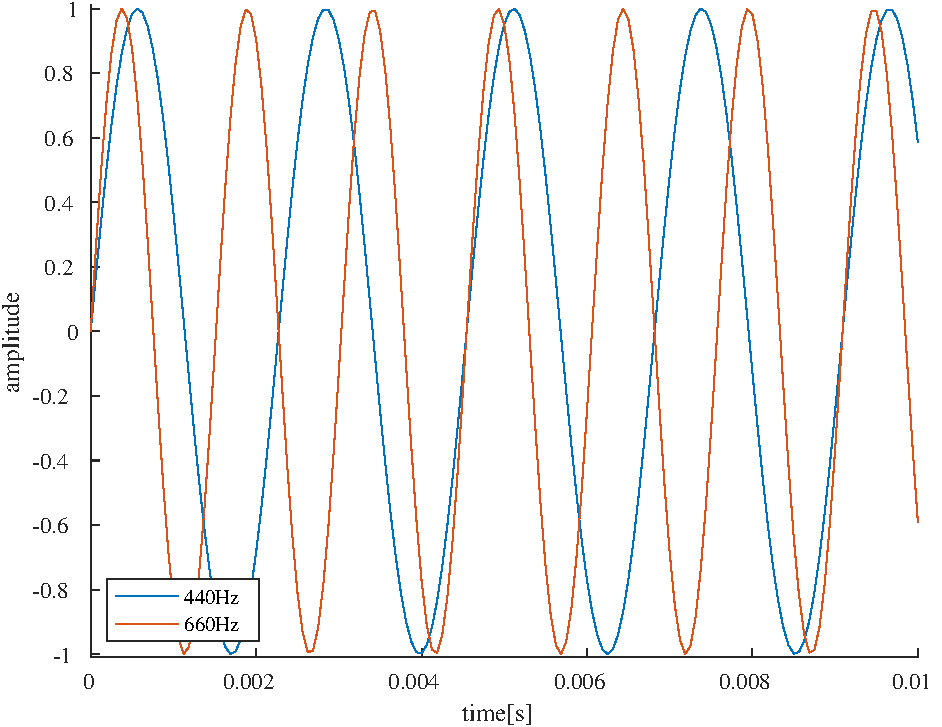
\includegraphics[keepaspectratio,width=.3\textwidth]{../../Figures/01_01.pdf}
    \caption{周波数が異なる正弦波のグラフ}
    \label{fig:\kadaiaa}
\end{wrapfigure}
さらに,聴音確認・目視確認では音の大きさ,音色,振幅や波形の変化は確認でなかった.\par
\consideration 周波数\ \((f)\)\ とは1秒間の振動回数であり,これが音の高さを決める.実験結果より周波数が大きい,つまり1秒間により多く振動すれば音が高くなることが分かった.
また,1回振動あたりの時間を周期\ \((T)\)\ と言うが,周期と周波数は反比例の関係であり,\eqref{equ:周期と周波数}が成り立つ.
\begin{align}
    f & =\frac{1}{T} & \big(\textrm{無論}\quad T\neq 0,\quad f\neq 0\big)\label{equ:周期と周波数}
\end{align}
\ref{fig:周波数の異なる純音の生成}より,周波数が大きい正弦波は周期が短く,逆もまた確認できる.
周波数のみを変更したので,振幅や正弦波の波形変化はない.\par
また,周波数が\(f_1\)正弦波の音と\(f_2\)正弦波の音はそれぞれ純音だがこれらの間にも関係がある.数学的には\(f_1:f_2=2:3\)の簡単な整数比になっている.
\begin{leftbar}
    ヒトの耳は2つの音を同時に聞いた場合,その2つの音の周波数が簡単になっているほど協和して聴こえる.(略)\par
    このように周波数比が整数比になっている音程を純音程とよぶ.\hfill{\cite[p.46-p.47]{音響工学理論基礎}}
\end{leftbar}
つまり,周波数\(f_1\)正弦波と周波数\(f_2\)正弦波の加算合成波はは協和してきこえる.
\section{\kadaiab}\label{sec:\kadaiab}
\purpose
音の大小は何によって決まるのだろうか.音の大小に関わる波の振幅や,波を構成する上で重要な初期位相を変化させ,変化の前後での音の違いを聞き取り,人間の耳に初期位相の変化や振幅の変化がどのように感じるか実験を通して考察する.
\method
時刻\(t\)に対して周波数\(f\)の正弦波は\eqref{equ:正弦波}で得られるが,その初期位相(\textit{initial phase})を\(\phi\)とすると,その正弦波は\eqref{equ:正弦波_初期位相}となる.
\begin{align}
    y & =\sin(2\pi ft+\phi)\label{equ:正弦波_初期位相}
\end{align}また,同様な正弦波:\eqref{equ:正弦波}の振幅を\(A\)倍して得られる正弦波は\eqref{equ:正弦波_振幅}となる.
\begin{align}
    y & =A\sin(2\pi ft)\label{equ:正弦波_振幅}
\end{align}
\begin{wrapfigure}{r}[0mm]{.4\textwidth}
    \begin{lstlisting}[caption={左右から別の音を出力},label={src:左右から別の音を出力},numbers={none}]
Fs = 16000; % サンプリング周波数
y1 = 音声データ1; % N行1列(左)
y2 = 音声データ2; % N行1列(右)
y = [y1 y2]; % N行2列 列結合を行う
sound(y, Fs); 
    \end{lstlisting}
\end{wrapfigure}
\paragraph{実験内容}この実験では,初期位相の変化と振幅の変化,それぞれ実験し変化前と変化後の音や波形の違いを発見する.周波数は\(f=440\textrm{Hz}\)とし,サンプリング周波数を\(\texttt{Fs}=16000\textrm{Hz}\)とする.
左から純音,右から波長や初期位相を変化させた音を再生するようにして(\ref{src:左右から別の音を出力}),音の変化を確認する.\srcref{sec:\kadaiab}{src:01_02}
\begin{table}[h]
    \caption{\kadaiab\ 実験内容}
    \label{tbl:\kadaiab_実験内容}
    \begin{tabularx}{\textwidth}{RCCR}
        \multicolumn{1}{c}{\textbf{実験対象}} & \multicolumn{1}{c}{\textbf{振幅(基準倍)}} & \multicolumn{1}{c}{\textbf{初期位相}} & \multicolumn{1}{c}{\textbf{生成される正弦波}} \\
        \hline
        純音                                  & 基準                                        & 基準                                  & \(y_0=\sin(2\pi ft)\)                         \\
        \hline
        \multirow{2}{*}{振幅}                 & \(0.5\)                                     & \(0\)                                 & \(y_1=0.5\times\sin(2\pi ft)\)                \\
                                              & \(0.25\)                                    & \(0\)                                 & \(y_2=0.25\times\sin(2\pi ft)\)               \\
        \hline
        \multirow{2}{*}{初期位相}             & \(1\)                                       & \(+\frac{\pi}{2}\)                    & \(y_3=\sin(2\pi ft+\frac{\pi}{2})\)           \\
                                              & \(1\)                                       & \(+\pi\)                              & \(y_4=\sin(2\pi ft+\pi)\)                     \\
        \hline
    \end{tabularx}
\end{table}
\result
聴音確認の結果を\ref{tbl:\kadaiab_実験結果},\ref{fig:振幅・位相の確認_結果_振幅}及び\ref{fig:振幅・位相の確認_結果_初期位相}に示す.振幅の変化について,振幅の変化に比例した音量変化を確認できたが,初期位相の変化による音の変化は確認できなかった.
\begin{table}[H]
    \caption{\kadaiab\ 実験結果}
    \label{tbl:\kadaiab_実験結果}
    \begin{tabularx}{\textwidth}{ccclR}
        \multicolumn{1}{c}{\textbf{実験対象}} & \multicolumn{1}{c}{\textbf{振幅(基準倍)}} & \multicolumn{1}{c}{\textbf{初期位相}} & \multicolumn{1}{c}{\textbf{生成される正弦波}} & \multicolumn{1}{c}{\textbf{純音との比較}} \\
        \hline
        純音                                  & 基準                                        & 基準                                  & \(y_0=\sin(2\pi ft)\)                         & \multicolumn{1}{c}{---}                   \\
        \hline
        \multirow{2}{*}{振幅}                 & \(0.5\)                                     & \(0\)                                 & \(y_1=0.5\times\sin(2\pi ft)\)                & 音量がおおよそ\(1/2\)に聞こえた.         \\
                                              & \(0.25\)                                    & \(0\)                                 & \(y_2=0.25\times\sin(2\pi ft)\)               & 音量がおおよそ\(1/4\)に聞こえた.         \\
        \hline
        \multirow{2}{*}{初期位相}             & \(1\)                                       & \(+\frac{\pi}{2}\)                    & \(y_3=\sin(2\pi ft+\frac{\pi}{2})\)           & 違いは分からなかった.                    \\
                                              & \(1\)                                       & \(+\pi\)                              & \(y_4=\sin(2\pi ft+\pi)\)                     & 違いは分からなかった.                    \\
        \hline
    \end{tabularx}
\end{table}
\begin{figure}[H]
    \centering
    \begin{minipage}[b]{.48\textwidth}
        \centering
        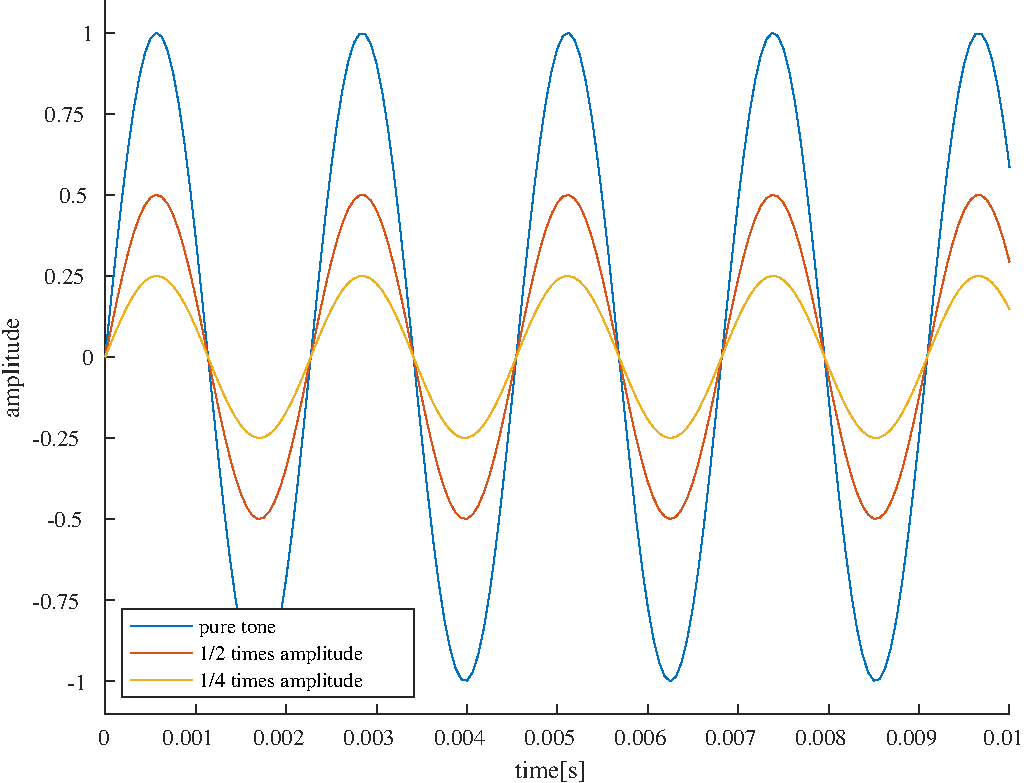
\includegraphics[keepaspectratio,width=\textwidth]{../../Figures/01_02_1.pdf}
        \caption{\kadaiab\ 実験結果(振幅の変化)}
        \label{fig:\kadaiab_結果_振幅}
    \end{minipage}
    \begin{minipage}[b]{.48\textwidth}
        \centering
        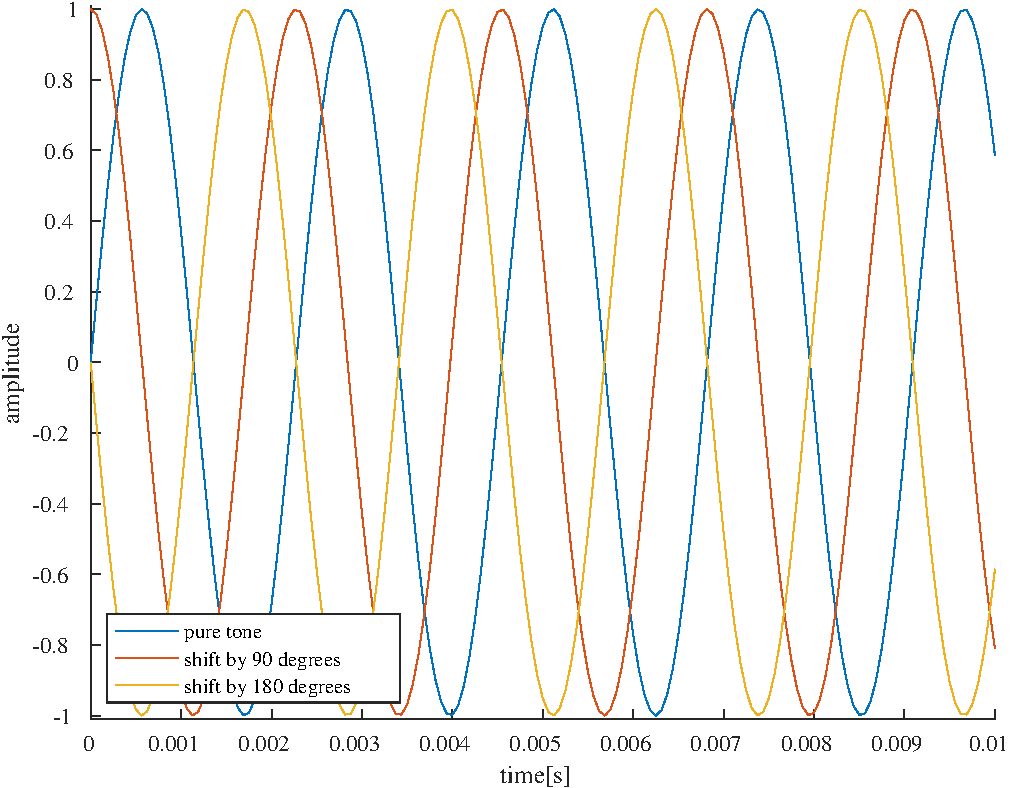
\includegraphics[keepaspectratio,width=\textwidth]{../../Figures/01_02_2.pdf}
        \caption{\kadaiab\ 実験結果(初期位相の変化)}
        \label{fig:\kadaiab_結果_初期位相}
    \end{minipage}
\end{figure}
\consideration
\paragraph{振幅の変化について} 振幅の変化は,音量と比例することを確認できた.\ref{fig:振幅・位相の確認_結果_振幅}より,各正弦波において周期や初期位相が等しいので,縦軸が\(0\)になる時刻や最大値を迎えるは等しいく,振幅のみが異なる.
\paragraph{初期位相の変化について} 位相の変化による音の変化は確認できなかった.\ref{fig:振幅・位相の確認_結果_初期位相}より,振幅や周期は等しいが,初期位相が異なるため最小値や最大値を迎える時刻が初期位相分異なる.
\section{\kadaiac}\label{sec:\kadaiac}
\purpose
ティンパニやギターのチューニングを行うとき,音叉やチューナーから音を出して,異なる互いに周波数であれば気づきチューニングする.それぞれ異なる周波数が異なる周波数が周波数の違いによるうなりの発生やその原因を数学的観点から考察する.
\method
うなりとは,異なる周波数が干渉するとき起こる現象である.異なる周波数同士の正弦波が干渉することで,強め合いの場所と弱め合いの場所が周期的に現れることで発生する.
例えば周波数\(f_1\)の正弦波に対して周波数\(f_2(\neq f_1)\)の正弦波を干渉させると,\eqref{equ:うなり}より\(1\)秒間に\(N\)回のうなりを聞くことができる.
\begin{align}
    N & = \big|f_1-f_2\big|\label{equ:うなり}
\end{align}
\(f_1\)と\(f_2\)の差が大きければ,当然うなり(\(N\))の回数は多くなり,\(f_1\)と\(f_2\)の差が小さければうなりの回数は少なくなる.\par
本実験では,サンプリング周波数を\(\texttt{Fs}=16000\textrm{Hz}\),提示時間\(4\)秒,周波数が\(f_1=440\textrm{Hz}\)の純音\(y_1\),\(f_2=441\textrm{Hz}\)の純音\(y_2\)を加算合成\(\big(y_1+y_2\big)\)した波形を生成し再生する.\srcref{sec:\kadaiac}{src:01_03}
\begin{wrapfigure}{r}[0mm]{.3\textwidth}
    \centering
    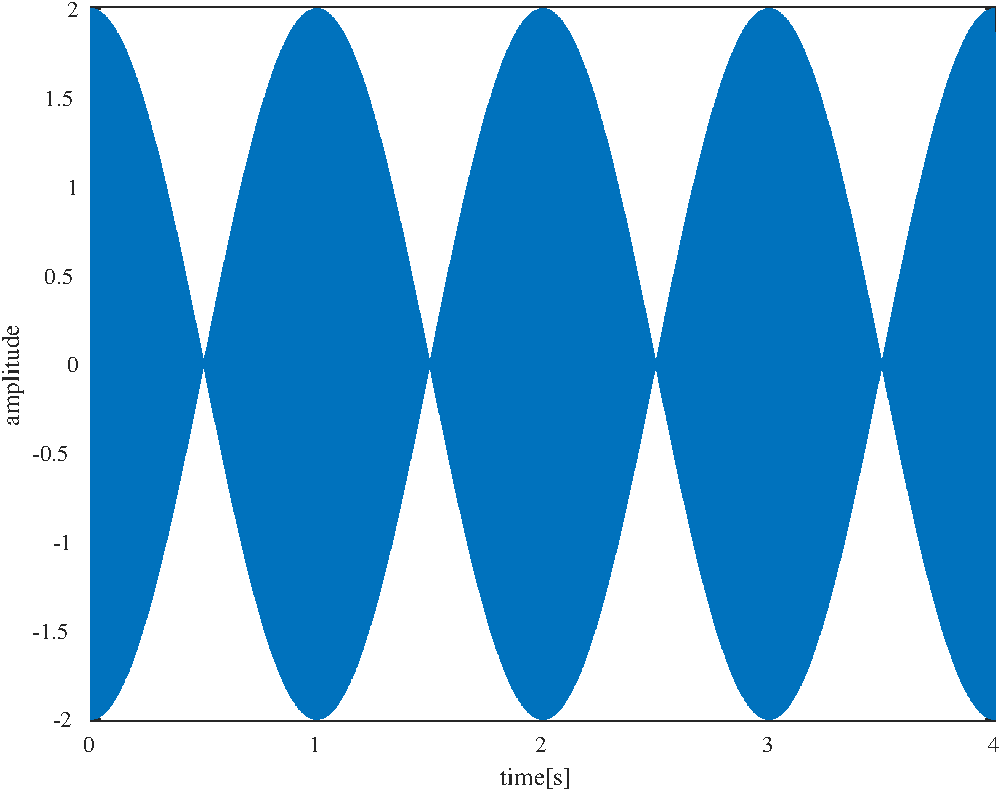
\includegraphics[keepaspectratio,width=.3\textwidth]{../../Figures/01_03.pdf}
    \caption{\kadaiac\ 実験結果}
    \label{fig:\kadaiac_実験結果}
\end{wrapfigure}
\result
うなりは4回聞こえた.また,時間軸に対して加算合成したデータを描画すると\ref{fig:\kadaiac_実験結果}となった.
\consideration \eqref{equ:うなり}に従って,
\begin{equation}
    \begin{aligned}
        \big|f_1-f_2\big| & = \big|440-441\big| \\
                          & =1
    \end{aligned}
\end{equation}
より\(1\)秒あたり\(1\)回のうなりが聞こえるはずなので,この実験結果は論理的に正しい.
加算合成波\ref{fig:\kadaiac_実験結果}の振幅に着目しても,周波数\(f_1\),\(f_2\)それぞれの正弦波の振幅が1であることを考えると,その加算合成波の振幅が2であることも理解できる.
さらに,この加算合成波は\(t=0\)のとき最大値を迎えており,これは初期位相が同一の正弦波の加算合成であることを表している.
\section{\kadaiad}\label{sec:\kadaiad}
\purpose
矩形波は周期関数だが,見た目は正弦波ではない.これをプログラム上でどのように再現するのか.フーリエ級数展開を用いた矩形波の描画やフーリエ級数展開のプログラム上で再現し,理想的な矩形波との比較を行う.
\method
\paragraph{フーリエ級数展開}周期\(T\)の任意の周期信号\(f(t)\)に対して,それはより短い周期\(T/n(n=1,2,\dots)\)を持つ正弦波の重ね合わせで表すことができる.具体的には\eqref{equ:フーリエ級数展開}の\(N=\infty\)で表すことができ,これをフーリエ級数展開という.\cite[p.18-p.19]{信号処理}特に\eqref{equ:フーリエ級数展開}の\(N=1\)の時を基本周波数と呼ぶ.
また,\(k>1\)のときの周波数を持つ正弦波を高調波と呼ぶ.

\begin{wrapfigure}{r}[0cm]{.3\textwidth}
    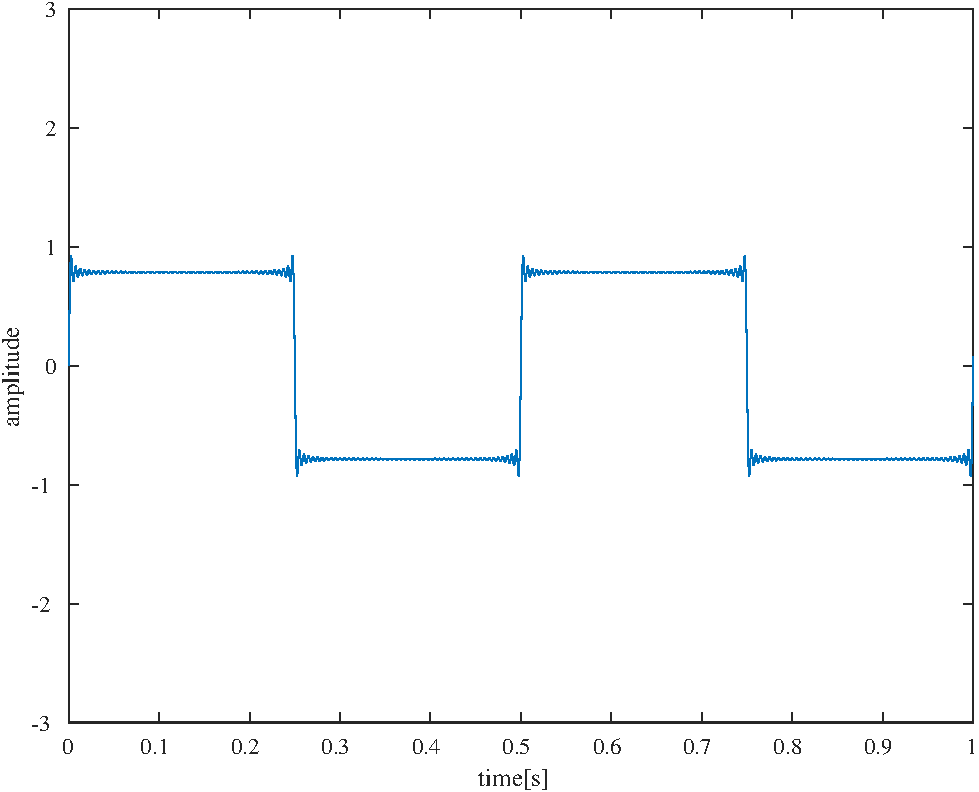
\includegraphics[keepaspectratio,width=.3\textwidth]{../../Figures/01_04_1.pdf}
    \caption{矩形波(\(1\leq k\leq 50\))}
    \label{fig:矩形波}
\end{wrapfigure}
\begin{align}
    f(t) & =\frac{1}{2}a_0 + \sum_{k=1}^{N}\big(a_k\cos(k\omega_0t)+b_k\sin(k\omega_0t)\big) & \omega_0 & =\frac{2\pi}{T}\label{equ:フーリエ級数展開}
\end{align}
\paragraph{矩形波}
矩形波は周期関数である.その周期を\(T\)とすると,関数\(f\)は時刻\(t\)に対して,フーリエ級数展開するとになる.\eqref{equ:矩形波}\((N=\infty)\)は周期\(T=1/2\)で定義した矩形波で,\eqref{equ:矩形波}を\(N=50\)で出力した.
\begin{align}
    f(t) & =\sum_{k=1}^{N}\frac{1}{2k-1}\sin\big(2\pi(2k-1)ft\big)\label{equ:矩形波}
\end{align}
\paragraph{実験内容}周期\(T=1/2\)として,\eqref{equ:矩形波}の\(N\)の値を\(N=1, 5, 25\)と増やした時に次第に波形が矩形波に収束していくことを確認する.
計算機で和\(\big(\sum\big)\)の演算をに示す通りに行う.\srcref{sec:\kadaiad}{src:01_04}
\begin{lstlisting}[caption={和の演算},label={src:和の演算},numbers={none}]
y = 0;
for k=1:50
    y = y + 1/(2*k-1) * sin(2*pi*(2*k-1)*f*t); % 矩形波の例
end
\end{lstlisting}
\result
\begin{wrapfigure}{r}[0mm]{.3\textwidth}
    \centering
    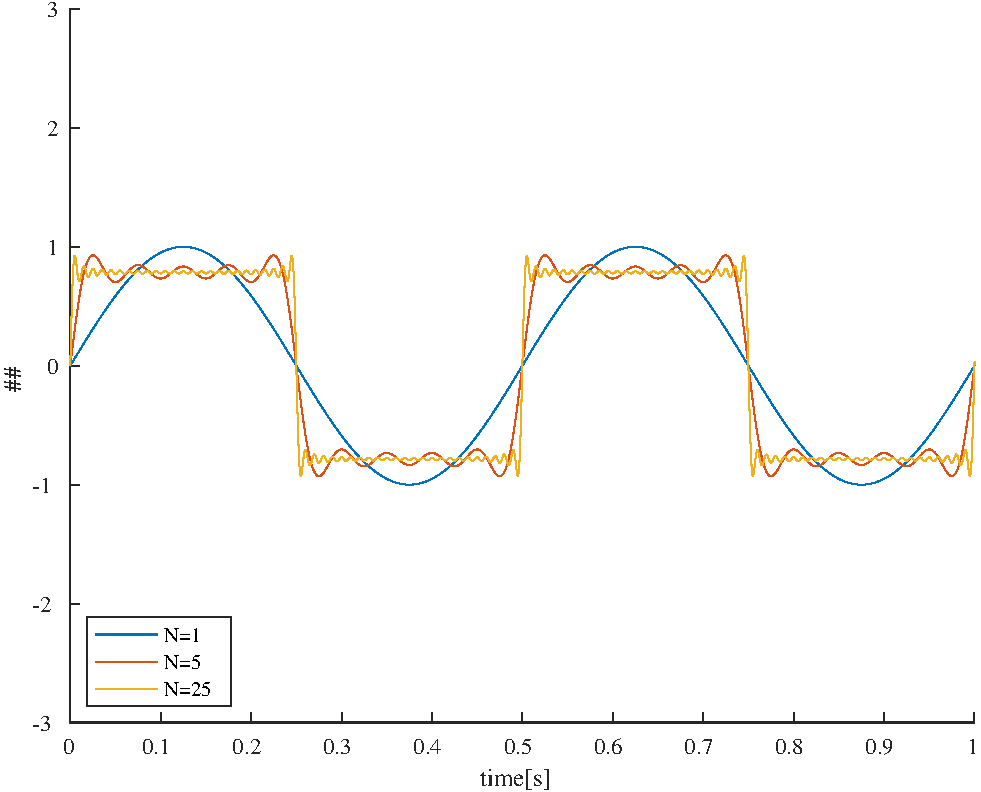
\includegraphics[keepaspectratio,width=.3\textwidth]{../../Figures/01_04_2.pdf}
    \caption{\kadaiad\ 実験結果}
    \label{fig:\kadaiae_実験結果}
    \vspace{-1cm}
\end{wrapfigure}
\ref{fig:\kadaiae_実験結果}の通り,\(N\)を大きくすると,矩形波に収束することがわかった.また,基本周波数と矩形波の周期も目測では一致している.
\consideration
計算機を用いて\(N\)の値を無限大で出力することは不可能である.\ref{fig:矩形波}のように\(N=50\)として出力すると,理想的な矩形波に近づくが完全ではない.\par
ここで\(N\)の値を大きくすると,\(T/2, T\)あたりで尖ったもの(ひげ)が確認される.フーリエ級数では不連続で誤差が大きい.このことをギブス現象という.\cite[p.34]{信号処理}
\section{\kadaiae}\label{sec:\kadaiae}
\purpose
白色雑音(\textit{white noise})は以下のように定義されている.
\begin{leftbar}
    すべての周波数成分を均等に含む,パワースペクトルが一定である不規則性の非常に強い波のことである.
    \hfill\cite{witenoise}
\end{leftbar}
ガウス雑音(\textit{gaussian noise})は以下のように定義されている.
\begin{leftbar}
    Gaussian noise represents statistical noise having the probability density function equal to that of the normal distribution.
    \hfill\cite{barbu2013variational}
\end{leftbar}
つまり,「正規分布の確率関数と等しい確率密度関数を持つ統計的ノイズ」を表す.今回の実験ではガウス雑音を計算機上で構成し,その信号振幅のヒストグラムを作成する.そのヒストグラムがガウス分布\footnote{以後,課題内容や他の用語との兼ね合いにより「正規分布」を「ガウス分布」と表す.}に従っているかを確認する.

\begin{wrapfigure}{r}[0mm]{.3\textwidth}
    \vspace{-.5cm}
    \begin{lstlisting}[caption={乱数生成・ヒストグラム},label={src:乱数生成・ヒストグラム},xleftmargin=3mm]
rng(0, 'twister');
X = randn(n,m);
num = 100;
[h, c] = hist(X, num);
plot(c,h);
    \end{lstlisting}
    \begin{lstlisting}[caption={平均と標準偏差の変更},label={src:平均と標準偏差の変更},numbers={none},xleftmargin=3mm]
X = randn(n,m); % 乱数生成
X = a.*X + b; % 演算
    \end{lstlisting}
    \vspace{-1cm}
\end{wrapfigure}
\method
\paragraph{\matlab 関数の説明}標準正規分布から乱数の行列を取り出すには,\texttt{randn}関数を用いる.乱数生成機の初期化を行い,\mat{n}{m}の乱数をを取り出すには,\ref{src:乱数生成・ヒストグラム}[1-2行目]を記述する.
また,データ列\texttt{X}に対して,ヒストグラムを\texttt{num}段階で分割し表示するためには,\ref{src:乱数生成・ヒストグラム}[3-5行目]を記述する.
\paragraph{ガウス分布と標準正規分布}ガウス分布とは,平均値・中央値・最頻値が一致するという特徴を持つ確率分布.その確率変数を\(x\)としたときの確率密度関数\(f\)は\eqref{equ:確率密度関数}のように与えらえる.
標準正規分布は,平均\(\mu=0\),標準偏差\(\sigma^2=1\)のガウス分布である.その標準正規分布の確率密度関数\(f_N\)は\eqref{equ:標準正規分布}となる.
\begin{align}
    f(x)   & = \frac{1}{\sqrt{2\pi\sigma^2}}\exp\left(-\frac{(x-\mu^2)}{2\sigma^2}\right) & \big(\mu:\textrm{平均}\quad\sigma^2:\textrm{分散}\quad-\infty<x<\infty\big)\label{equ:確率密度関数} \\
    f_N(x) & =\frac{1}{\sqrt{2\pi}}\exp\left(-\frac{x^2}{2}\right)                        & \big(-\infty<x<\infty\big)\label{equ:標準正規分布}
\end{align}
\begin{leftbar}
    確率変数\(x\)に対して,その平均が\(\mu_x\),分散が\({\sigma_x}^2\)のとき,\(y=ax+b\quad(a\textrm{と}b\textrm{は定数})\)で定義される確率変数\(y\)の平均は\(\mu_y=a\mu_x+b\),分散は\({\sigma_y}^2=a^2{\sigma_x}^2\)となる.\hfill\cite{matlab}
\end{leftbar}
従って,標準正規分布に従って出力されたデータ列の平均を\texttt{a},標準偏差を\texttt{b}に変更したい場合には,\mat{n}{m}データ列\texttt{X}に対して\texttt{X}の各要素と\texttt{a}の積をとり,データ列\texttt{X}と\texttt{b}の和をとる.(\ref{src:平均と標準偏差の変更})\srcref{sec:\kadaiae}{src:01_05}
\result
ガウス雑音の波形を\ref{fig:ガウス雑音の波形},ヒストグラムを\ref{fig:ヒストグラム}に示す.聴音した結果,「ザー」という所謂雑音が聞こえた.
\begin{figure}[h]
    \centering
    \begin{minipage}[b]{.48\textwidth}
        \centering
        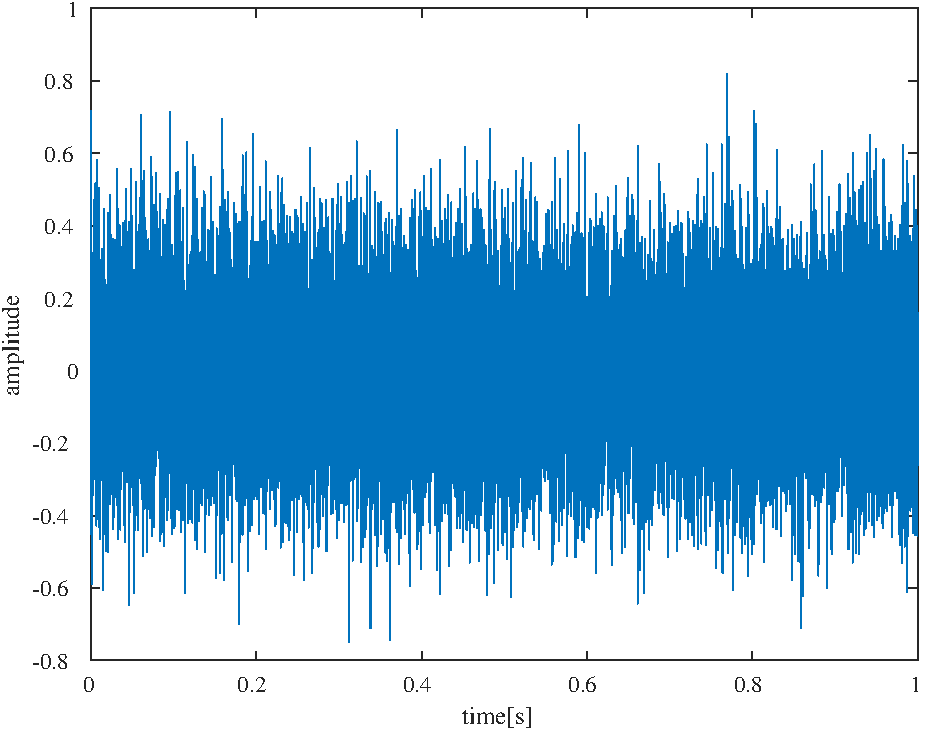
\includegraphics[keepaspectratio,height=.2\textheight]{../../Figures/01_05_0.pdf}
        \caption{ガウス雑音の波形}
        \label{fig:ガウス雑音の波形}
    \end{minipage}
    \begin{minipage}[b]{.48\textwidth}
        \centering
        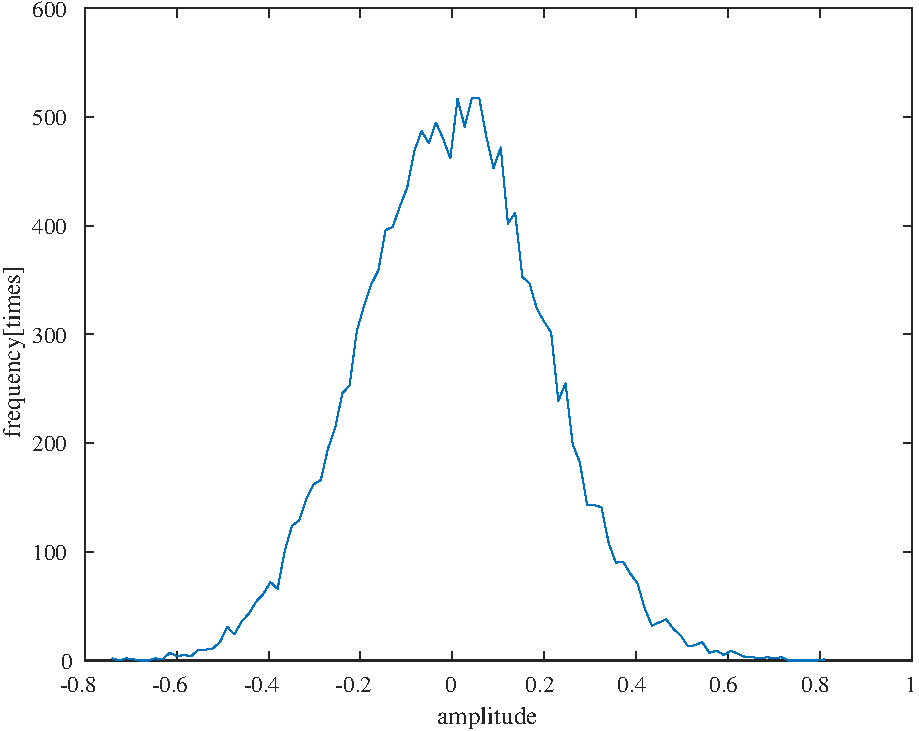
\includegraphics[keepaspectratio,height=.2\textheight]{../../Figures/01_05_1.pdf}
        \caption{ヒストグラム}
        \label{fig:ヒストグラム}
    \end{minipage}
\end{figure}
\consideration
聴音確認による,ガウス雑音の特徴は捉えることができなかった.ヒストグラム\ref{fig:ヒストグラム}を確認すると,平均\(\mu=0\)のガウス分布におおよそ従っていることがわかる.

\chapter{\kadaib}
\section{\purpose}
この実験では,画像に対してフィルタの適用や色空間を変換する.\par
\paragraph{画像フィルタ} 画像に対して,フィルタを適用するとはどのようなことか?我々は,携帯電話の写真アプリケーションを用いて,写真を「加工」する.
我々は「加工」という行為を「フィルタをかける」と呼ぶが,この「フィルタ」という言葉と,画像処理におけるフィルタは意味が異なる.
画像処理におけるフィルタは,画像ないに含まれる雑音を除去したり,特徴を抽出したりすることで欠陥検出をより円滑に行うための基本処理を指す\cite{画像フィルタ}.
\newcommand{\originimg}{\texttt{original\_img}}
テスト画像として,以下の画像を用意する.元画像を\originimg とする.
\setlength{\columnseprule}{0.1mm}
\begin{enumerate}
    \item \textbf{白色ガウス雑音}\\
          \newcommand{\wgnimg}{\texttt{wgn\_img}}
          白色ガウス雑音は,白色性を持つガウス雑音である.今回は,平均\(0\),標準偏差\(10\)としてガウス分布の乱数を発生させる.
          このテスト画像を\wgnimg とする.
    \item \textbf{インパルス雑音}\\
          \newcommand{\inimg}{\texttt{in\_img}}
          インパルス雑音とは.超短時間におこる高周波の雑音のことを指す.今回は,画像のランダムな画素を,白または黒で塗り替える.それぞれ全体画素の1\% の割合で作成する.
          このテスト画像を\inimg とする.
\end{enumerate}
画像フィルタはいくつかの種類があり,画像雑音の除去やエッジの強調に用いられる.
\begin{enumerate}
    \item \textbf{平滑化フィルタ}
          \begin{itemize}
              \item 画像の各画素\(p\)に対して,\(n\)近傍と中央の画素値の平均や重み付け平均をとり,\(p\)の画素値とするフィルタ.
              \item 今回の実験では,各画素\(p\)に対して,\(3\times 3\),つまり8近傍と\(p\)の画素値の平均をとり,中央の画素値として定義する.2つのテスト画像にフィルタを適用し,雑音とフィルタの関係を考察する.
          \end{itemize}
    \item \textbf{メディアンフィルタ}
          \begin{itemize}
              \item 画像の各画素\(p\)に対して,\(n\)近傍と中央の画素値を昇順に整列し,その中央値を\(p\)の画素値とする.
              \item 今回の実験では,各画素\(p\)に対して,\(3\times 3\),つまり8近傍と\(p\)の画素値を昇順に整列する.その中央値を\(p\)の画素値として定義する.2つのテスト画像にフィルタを適用し,雑音とフィルタの関係を考察する.
          \end{itemize}
    \item \textbf{微分フィルタ}
          \begin{itemize}
              \item 微分フィルタは,境界線の強調や局所的な特徴の抽出するフィルタである.しかし,一次微分フィルタ,二次微分フィルタを用いると,画像の雑音も強調される.ここでPrewittフィルタとSobelフィルタを用いると,雑音がある画像でもうまく境界線を抽出できる\cite[p.87]{画像処理}.
                    \begin{itemize}
                        \item \textbf{Prewitt Filter}:隣り合う2画素の画素値を持ちいて3画素ずつをセットにして濃度の変化点を抽出するアルゴリズム\cite[p.87]{画像処理}.
                        \item \textbf{Sobel Filter}:画像の各ピクセルの周囲の画素との差を計算して,その差の大きさを使って,エッジを検出するアルゴリズム.
                    \end{itemize}
              \item 今回の実験では,\originimg に対して,Sobelフィルタを用いて縦微分,横微分,縦微分と横微分の加算合成した画像を作成する.フィルタを適用した画像の特徴と,それぞれの違いを考察する.
          \end{itemize}
    \item \textbf{ラプラシアンフィルタ}
          \begin{itemize}
              \item ラプラシアンフィルタは,微分フィルタ同様,境界線を見つけるために使われる方法である.
              \item 今回の実験では,\originimg に対して,ラプラシアンフィルタを適用し,適用した画像と特徴と違いを考察する.
          \end{itemize}
\end{enumerate}
\begin{figure}[h]
    \centering
    \begin{minipage}[b]{.24\textwidth}
        \centering
        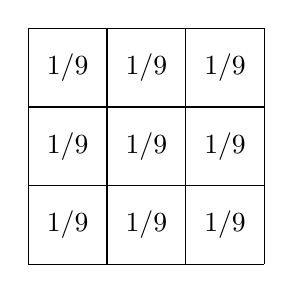
\begin{tikzpicture}
            \draw (0,0) grid (3,3);
            \foreach \u \v in {0.5/0.5,1.5/0.5,2.5/0.5,0.5/1.5,1.5/1.5,2.5/1.5,0.5/2.5,1.5/2.5,2.5/2.5}
            \node at (\u,\v) {\(1/9\)};
        \end{tikzpicture}
        \subcaption{平滑化フィルタ}
        \label{fig:平滑化フィルタ}
    \end{minipage}
    \begin{minipage}[b]{.24\textwidth}
        \centering
        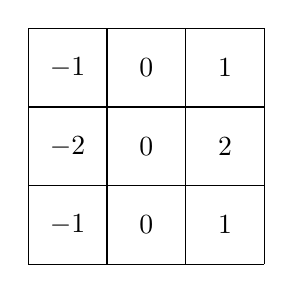
\begin{tikzpicture}
            \draw (0,0) grid (3,3);
            \foreach \u \v \w in {0.5/0.5/{\(-1\)},1.5/0.5/{\(0\)},2.5/0.5/{\(1\)},0.5/1.5/{\(-2\)},1.5/1.5/{\(0\)},2.5/1.5/{\(2\)},0.5/2.5/{\(-1\)},1.5/2.5/{\(0\)},2.5/2.5/{\(1\)}}
            \node at (\u,\v) {\w};
        \end{tikzpicture}
        \subcaption{Prewittフィルタ:横方向}
        \label{fig:Prewittフィルタ_横方向}
    \end{minipage}
    \begin{minipage}[b]{.24\textwidth}
        \centering
        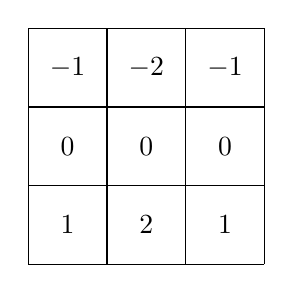
\begin{tikzpicture}
            \draw (0,0) grid (3,3);
            \foreach \u \v \w in {0.5/0.5/{\(1\)},1.5/0.5/{\(2\)},2.5/0.5/{\(1\)},0.5/1.5/{\(0\)},1.5/1.5/{\(0\)},2.5/1.5/{\(0\)},0.5/2.5/{\(-1\)},1.5/2.5/{\(-2\)},2.5/2.5/{\(-1\)}}
            \node at (\u,\v) {\w};
        \end{tikzpicture}
        \subcaption{Prewittフィルタ:縦方向}
        \label{fig:Prewittフィルタ_縦方向}
    \end{minipage}
    \begin{minipage}[b]{.24\textwidth}
        \centering
        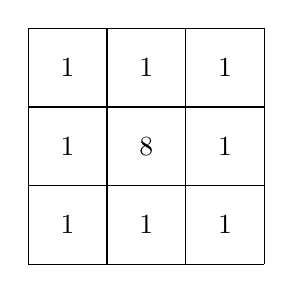
\begin{tikzpicture}
            \draw (0,0) grid (3,3);
            \foreach \u \v in {0.5/0.5,1.5/0.5,2.5/0.5,0.5/1.5,2.5/1.5,0.5/2.5,1.5/2.5,2.5/2.5}
            \node at (\u,\v) {\(1\)};
            \node at (1.5,1.5) {\(8\)};
        \end{tikzpicture}
        \subcaption{ラプラシアンフィルタ}
        \label{fig:ラプラシアンフィルタ}
    \end{minipage}
    \caption{\(3\times 3\)画像フィルタ}
\end{figure}
\paragraph{色空間変換}この実験では,RGB色空間から,HSV色空間へ変換する.RGB色空間は,赤(Red),緑(Green),青(Blue)の3チャネルで構成する.HSVは色相(Hue),彩度(Saturation),明度(Value)の3チャネルで構成する.
HSV色空間の特徴として,人間が色を知覚する方法と類似しており,視覚障害者向けのアクセシビリティ向上に役立つことが挙げられる.たとえば,HSVの「明度」を調節することで,文字が見やすくなる\cite[p.97\ -\ p.98]{画像処理}.\par
また,人間が色を知覚する方法と類似していることを踏まえて,HSV色空間を用いることで,画像の特徴を抽出しやすくなる.
今回の実験では,自分の手の写真をRGB色空間からHSV色空間へ変換し,肌色領域を抽出する.抽出した肌色領域を白色,そのほかの部分を黒色にして出力する.出力した画像と,RGB色空間における肌色領域を抽出した場合の精度について考察する.
\bibliography{bib}
\chapter*{付録}
\pagestyle{appendixstyle}
\addcontentsline{toc}{chapter}{付録}
\setcounter{section}{0}
\renewcommand{\thelstlisting}{\thesection-\arabic{lstlisting}}
\renewcommand{\thesection}{\Alph{section}}
\newcommand{\secref}[1]{[#1]{#1}}
\makeatletter
\@addtoreset{lstlisting}{section}
\makeatother
\lstset{
    frame={single},
    numbers={left}
}
\section{\kadaia\ (April 27th, 2023)}
\lstinputlisting[caption={\secref{\kadaiaa}},label={src:05_01}]{../../05_UnderstandingImages/no1.m}
\lstinputlisting[caption={\secref{\kadaiab}},label={src:05_02}]{../../05_UnderstandingImages/no2.m}
\lstinputlisting[caption={\secref{\kadaiac}},label={src:05_03}]{../../05_UnderstandingImages/no3.m}
\lstinputlisting[caption={\secref{\kadaiad}},label={src:05_04}]{../../05_UnderstandingImages/no4.m}
\lstinputlisting[caption={\secref{\kadaiae}},label={src:05_05}]{../../05_UnderstandingImages/no5.m}
\lstinputlisting[caption={\secref{\kadaiaf}},label={src:05_06}]{../../05_UnderstandingImages/no6.m}
\section{\kadaib\ (May 8th, 2023)}
\lstinputlisting[caption={\secref{\kadaiba}},label={src:06_01}]{../../06_ImageFiltering/no1.m}
\lstinputlisting[caption={\secref{\kadaibb}},label={src:06_02}]{../../06_ImageFiltering/no2.m}
\lstinputlisting[caption={\secref{\kadaibc}},label={src:06_03}]{../../06_ImageFiltering/no3.m}
\lstinputlisting[caption={\secref{\kadaibd}},label={src:06_04}]{../../06_ImageFiltering/no4.m}
\lstinputlisting[caption={\secref{\kadaibe}},label={src:06_05}]{../../06_ImageFiltering/no5.m}
\lstinputlisting[caption={\secref{\kadaibd}\ \texttt{fucntion}},label={src:06_05_f}]{../../06_ImageFiltering/no5_hsvfunc.m}
\section{\ (April 20th, 2023)}
\section{\ (April 24th, 2023)}
\end{document}